\documentclass[acmtog, authorversion]{acmart}

\usepackage{booktabs} % For formal tables
\usepackage{hyperref}

% TOG prefers author-name bib system with square brackets
\citestyle{acmauthoryear}
\setcitestyle{square}

\usepackage[ruled]{algorithm2e} % For algorithms
\renewcommand{\algorithmcfname}{ALGORITHM}
\SetAlFnt{\small}
\SetAlCapFnt{\small}
\SetAlCapNameFnt{\small}
\SetAlCapHSkip{0pt}
\IncMargin{-\parindent}

% Metadata Information
\acmYear{2017}
\acmMonth{9}

% Copyright
%\setcopyright{acmcopyright}
%\setcopyright{acmlicensed}
\setcopyright{rightsretained}
%\setcopyright{usgov}
%\setcopyright{cagov}
%\setcopyright{cagovmixed}

% Document starts
\begin{document}
% Title portion
\title{Finding trends in open-source software by visualizing collaboration and influence over time}

\author{Rick Proost}
\affiliation{%
\institution{Delft University of Technology}
\country{The Netherlands}}
\email{rpjproost@gmail.com}

\author{Vincent Robbemond}
\affiliation{%
\institution{Delft University of Technology}
\country{The Netherlands}}
\email{vincentrobbemond@gmail.com}

\author{Wim Spaargaren}
\affiliation{%
\institution{Delft University of Technology}
\country{The Netherlands}}
\email{wim_spaargaren@live.nl}

\begin{abstract}
The open-source software community has seen a lot of growth in the past years and remains to grow.
Collaboration platforms like GitHub provide easy access to all open-source project data by providing an API, making data accessible for over 24 million users  \cite{GHOctoverse} .
While this data has been available for some time, there has not been done a lot of research into how this data can be applied to bring insights in the way developers collaborate.
Developer collaboration has become a bigger point of discussion since the rise of Globally Distributed Software Engineering and can benefit from insights derived from this readily available data.
This paper describes the building of an online platform to provide open source software collaboration visualizations on GitHub.
In addition, the evolution of developer activity for open source software projects  is explored.
This exploratory research is done by answering questions about the evolution of developer activity in the developer community and the way geographic distance between repository owner and developer influences the amount of commits made by a developer.
\end{abstract}

\keywords{Data Visualization, GitHub, Open Source Software, Collaboration}

\maketitle

\section{Introduction}
In the past few years the open-source software(OSS) community and development in OSS have grown.
According to GitHub \cite{GHOctoverse}, in 2016, there were over 5.8 million users engaged in activities relating to public repositories.
GitHub defines these activities as "some activity within the last year, e.g. code committed, a comment created, a repository starred, or an issue opened".

With GitHub providing programmatic access to all OSS repository and user data\cite{GHAPI}, it is possible to collect and manipulate this data to get more insights into the way the OSS community collaborates (on GitHub).
These new insights can then be applied to to e.g. develop new software development methods, improve existing (collaboration) platforms (like GitHub) or coding standards, which improve developer collaboration \cite{Jermakovics2013}.
Outside of the OSS community, a better understanding of how the OSS community functions helps commercial IT projects adopt typical OSS practices, e.g. promoting open collaboration \cite{Kalliamvakou:2015:OSC:2818754.2818825}, and may help IT planners make more informed decisions and develop more effective strategies for using OSS software \cite{madey2002}.

One way for researchers to analyze the gathered data, is by visualizing it \cite{Heller}.
One of the objective of the Software Visualization field is to aid stakeholders in developing a greater understanding of software systems, their evolution and development.
"The basic idea of visual data exploration is to present the data in some visual form, allowing the human to get insight into the data, draw conclusions, and directly interact with the data.
Visual data mining techniques have proven to be of high value in exploratory data analysis and they also have high potential for exploring large databases." \cite{981847}.
To give developers insights in repositories, GitHub also provides some visualizations, one of these visualization is "Developer Contribution", which shows amount of commits made during a period of time.
Up until now there have not been a lot of tools or platforms which provide visual insight into e.g. collaboration over time on a specific repository.
Tools which are available are outdated \cite{Heller} or not sufficient, for example a visualization of GitHub's newest and most popular repositories \cite{donnemartin2016}, a GitHub repository history visualizer \cite{artzub2013}, and a repository stats visualizer \cite{bajaj2013}.
Although these examples are visualization tools for GitHub, they provide insufficient information on developer collaboration in OSS projects.

Therefore, the main contribution of this paper is to provide a tool which stakeholders can leverage to gain insights into OSS projects and developer collaboration.
For example, available data will show where developers are located, this will help identifying possible cultural differences between collaborators which is important to prevent co-ordination and collaboration problems \cite{Mishra2014}.

The research question this paper will explore is: \textbf{Is it possible to find different patterns in OSS development by visualizing collaboration over time?}

Since this is a broad subject, we will explore this subject by answering two related, more specific, questions with the help of the aforementioned tool.
Answers to the related questions will not provide a conclusive answer to the main question asked but in turn invite others to extend and explore this subject.

GitHub statistics show that 24 million people are making use of GitHub, these users are divided over 200 countries in all continents, with Asia (7.1 million), North-America (5.9 million) and Europe (5.3 million) hosting the largest amount of users \cite{GHOctoverse}.
StackOverflow developer survey 2017 \cite{StackOverflow2017} has similar results, showing big clusters in the USA, Western-Europa and India.
Countries with the highest numbers of new users on GitHub are the USA (1.2 million) and China (0.7 million) \cite{GHOctoverse}.
It is no surprise that different countries have different growth rates of GitHub users, identifying and looking into countries with the highest growth rates could lead to interesting insights.
For example (IT) companies, identifying countries with a high growth in software developers is important since there has been a developer shortage for years and companies are competing for the best and brightest.
By adding a temporal element to active number of developers per country, it will be possible to tell in which countries the number of active developers in open-source software evolves faster.
Analyzing the trend in developer growth can then be leveraged by OSS stakeholders, for example companies seeking open-source developers to outsource software development to \cite{haefliger2008code}.

Underlying reasons can then be researched for this rise in popularity.

Therefore we first explore the question: \textbf{Does the number of active developers in the OSS community evolve faster for different countries?}

The second area we explore is developer collaboration, by analyzing collaboration links.
Collaboration links are defined as links between developers who add contributions consecutively to the same project.
By adding a temporal component to visualizing collaboration links, it becomes possible to see the way developer collaboration changes over time.
At the same time it becomes possible to see if the distance between developers working on the same project has influence on collaboration, and further exploring the impact of cultural differences in software development\cite{Mishra2014}.

The second question we explore is: \textbf{Does the number of commits made by a developer evolve faster for different countries?}

The answers could be derived from visualizing the data in such a way researchers can make well substantiated and testable hypotheses.
Therefore, the main outcome is that a service was developed that visualizes evolution on collaboration over time for development.

\section{Related work}
TODO
\cite{Jermakovics2013}
\cite{GHOctoverse}
\cite{StackOverflow2017}

\section{Methodology}
To answer the research questions,  a set of large repositories (i.e. repositories with the most GitHub stars and/or collaborators) on the open source software platform GitHub have been chosen.
A data scraper is built to retrieve data from the previously mentioned repositories.
The scraped data includes (but is not limited to) the owner, contributors and collaborators of the repository.
Aside from user information, commits are gathered for the repositories to compare statistics in different time frames.

A web-based service is created to efficiently search and navigate repositories or GitHub users.
Data gathered can then be displayed in multiple forms like geolocations for collaborators on an interactive map (e.g. Mapbox \cite{MapBox}) and activity for a project in a graph with a temporal component.
Different ways of linking users and repositories is experimented with and results are published and available online at \cite{githubvisualizerovertime}.

By creating this web-based service, new insights will emerge for collaboration in open source software development.
Trends in software collaboration, activity and collaboration links over time will be revealed.
In addition, a new way is provided for researchers to retrieve insights in open source software development collaboration statistics and form new hypotheses by analyzing the dynamic visualizations.

\section{Implementation}
The first step in answering the research questions, is the retrieval of data from the software development platform GitHub.
This data is gathered by using the GitHub REST API\cite{GHAPI}.
The repositories retrieved are limited to the top 1000 starred repositories on GitHub, for two reasons:
First, according to Octoverse \cite{GHOctoverse} in 2016 there were nearly 20 million software repositories, storage of this amount of data goes beyond the scope of this research paper.
The second reason to choose the most starred repositories, is that stars give an indication to the popularity of a repository and therefore have higher chances on relatively more activity than less popular repositories.
The top 1000 starred repositories were listed and specified at \cite{gitstar} on september 2017.
Data for these projects was retrieved by a custom data scraper, the database dump can be found at  \cite{githubvisualizerovertime}.
The scraper first retrieved the repository data using the projects resource\cite{GHAPI}, afterwards all the commits with it’s user and at last location was translated into geocoordinates.
The GitHub platform allows a user to specify a location on their profile, which is stored as plain text.
This means not all users have a location and some locations may not be as specific as others.
Commit data contains a message which is mostly used to describe the change and a timestamp denoting commit time.
Commit author and committer data is also available, therefore it is possible to make a distinction if necessary.
Finally, another custom scraper retrieved all star events for each repository using the repository stargazer resource\cite{GHAPI}.
A stargazer is a user who starred a certain repository, so Developer A stars Repository B, therefore A is now in the list of stargazers of B.
The star events depict another way of activity in open source software development and can be of value when visualizing activity data.

TODO: Front-end features


\section{Evaluation}
TODO: Top 1000 starred projects are not updated

\section{Results}
The self developed data scraper can be found at \cite{githubvisualizerovertime} together with a database dump for the top 1000 starred repositories of September 2017.
This Golang scripts provide functionality to gather both commits and stars for projects.
Projects which data needs to be retrieved for, can be specified in two ways, by providing a json file with project names, or by reading repository names from a self provided database.
For each project, commits and stars from the current date until the last stored commit in the database will be retrieved and stored in the specified database.
Detailed build instructions are provided in the README file.
\begin{figure}
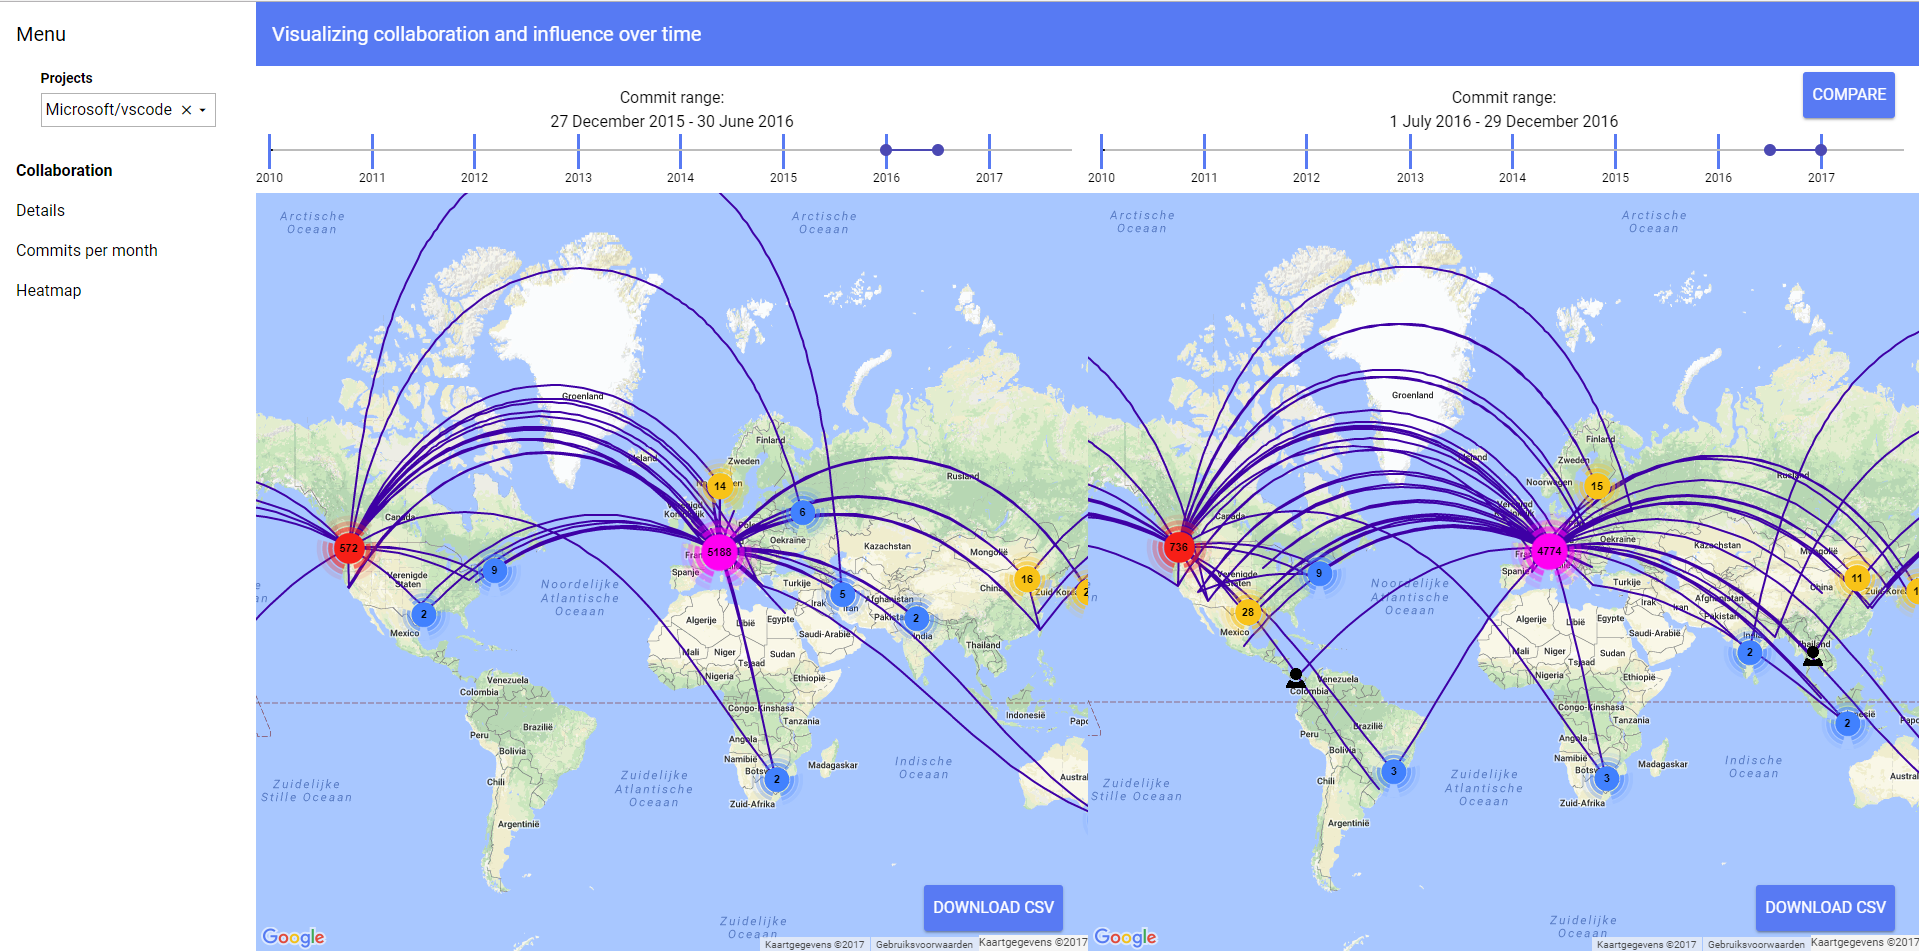
\includegraphics[scale=0.18]{images/vscode-compare.PNG}
\caption{Example visualization of developer collaboration comparison for VSCode}
\label{fig:collaboration}
\end{figure}

Figure ~\ref{fig:collaboration} shows a visualization example for the repository Visual Studio Code.
Markers depict commits, with a location of where the author of the commit is located.
Lines depict collaboration between developers.
This collaboration is defined as successive commits done by collaborators working on the same project.
When at a lower zoom level, nodes get un-grouped and lines between individual developers will be shown.
In the top of the page a timeline is shown.
In the timeline a timespan can be selected.
After selecting a timespan, commits within this timespan are shown on the map.
A download CSV button is added to download the shown commit data as CSV file.
This way users of the platform can further analyze the data shown.
By pressing the compare button, two visualizations can be shown next to each other.
In figure  ~\ref{fig:collaboration} commits from the first half of 2016 are compared to commits of the second half of 2016.
\begin{figure}
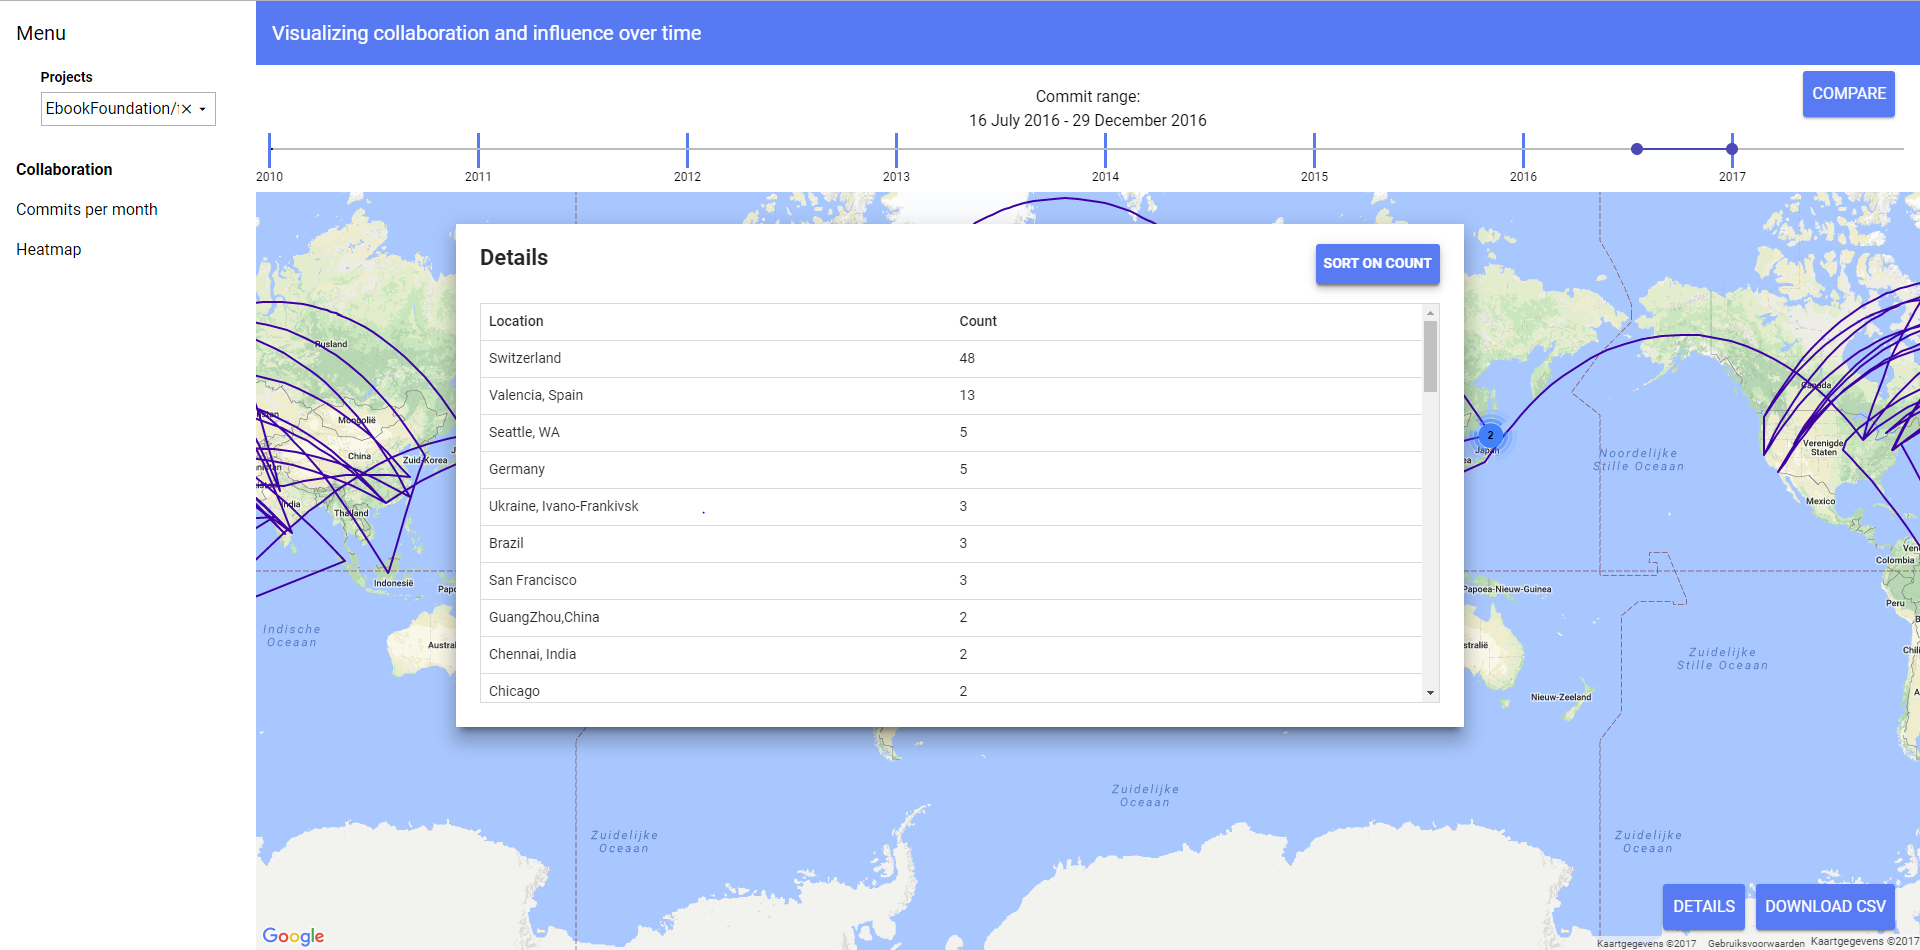
\includegraphics[scale=0.18]{images/details-popup-ebook-foundation.PNG}
\caption{Example details popup}
\label{fig:details}
\end{figure}

A second button is provided to show details about the commits currently shown on the map. 
By pressing the details button, a dialog is created with information about the number of commits per location, as shown in ~\ref{fig: details}.
In this example commits of the second half of 2016 are shown. 
In the dialog a sort on count button is added to sort the commit details in ascending or descending order.

\begin{figure}
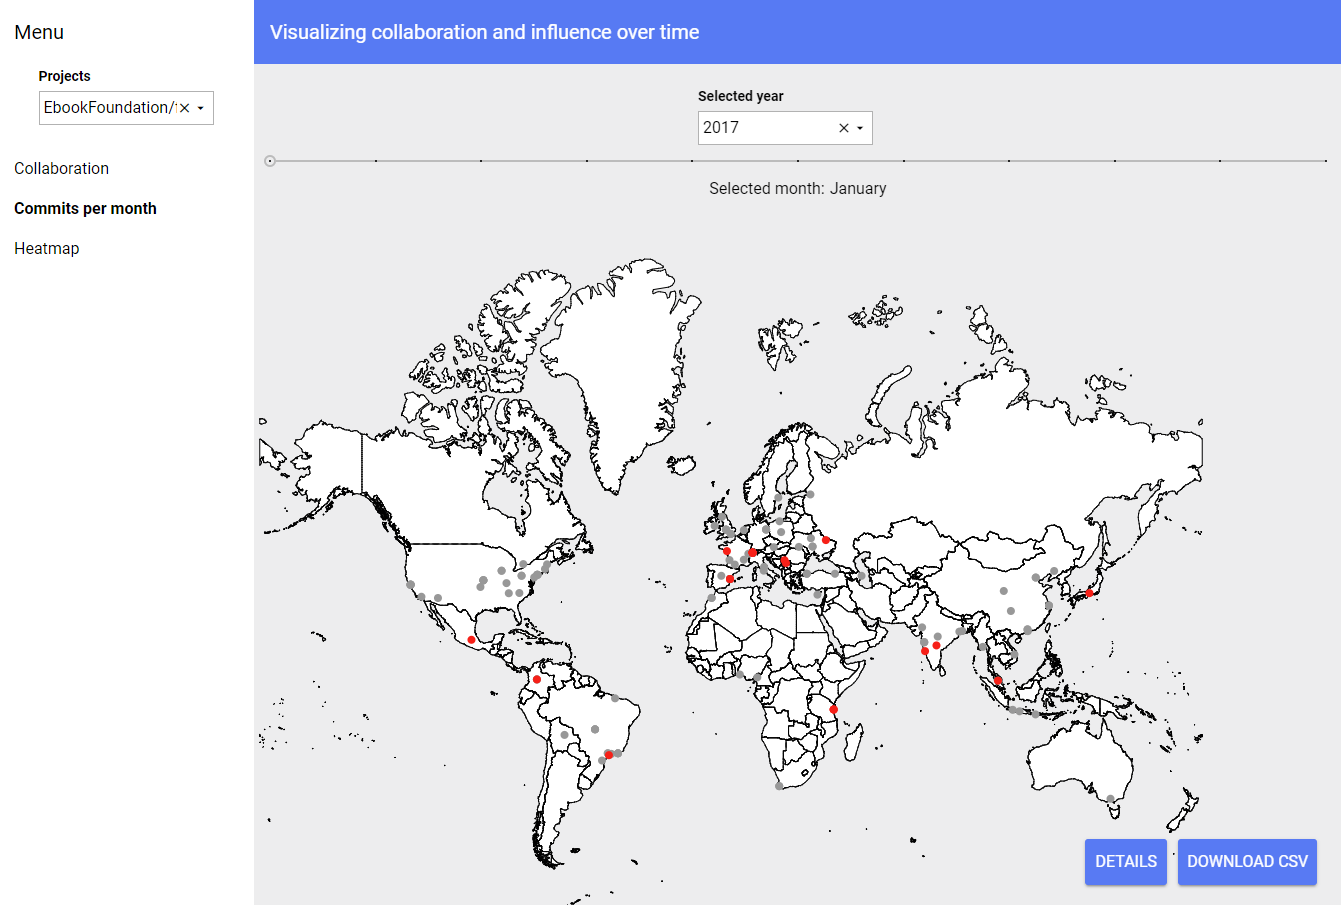
\includegraphics[scale=0.25]{images/d3-example-rails.PNG}
\caption{Example visualization of commits per month}
\label{fig:commits-period}
\end{figure}

Figure ~\ref{fig:commits-period} shows an example of a map built with the D3 library.
Every dot represents a commit belonging to a repository in a year span, which can be selected by selecting a year in the dropdown menu.
Red dots represent commits made during the month selected in the second slider.
Beneath this slider the selected month is stated.
By adjusting the month slider, it is possible to visualize how commits change per month for a project.
As well as the first visualization the details button as well as the download csv button are provided.

\begin{figure}
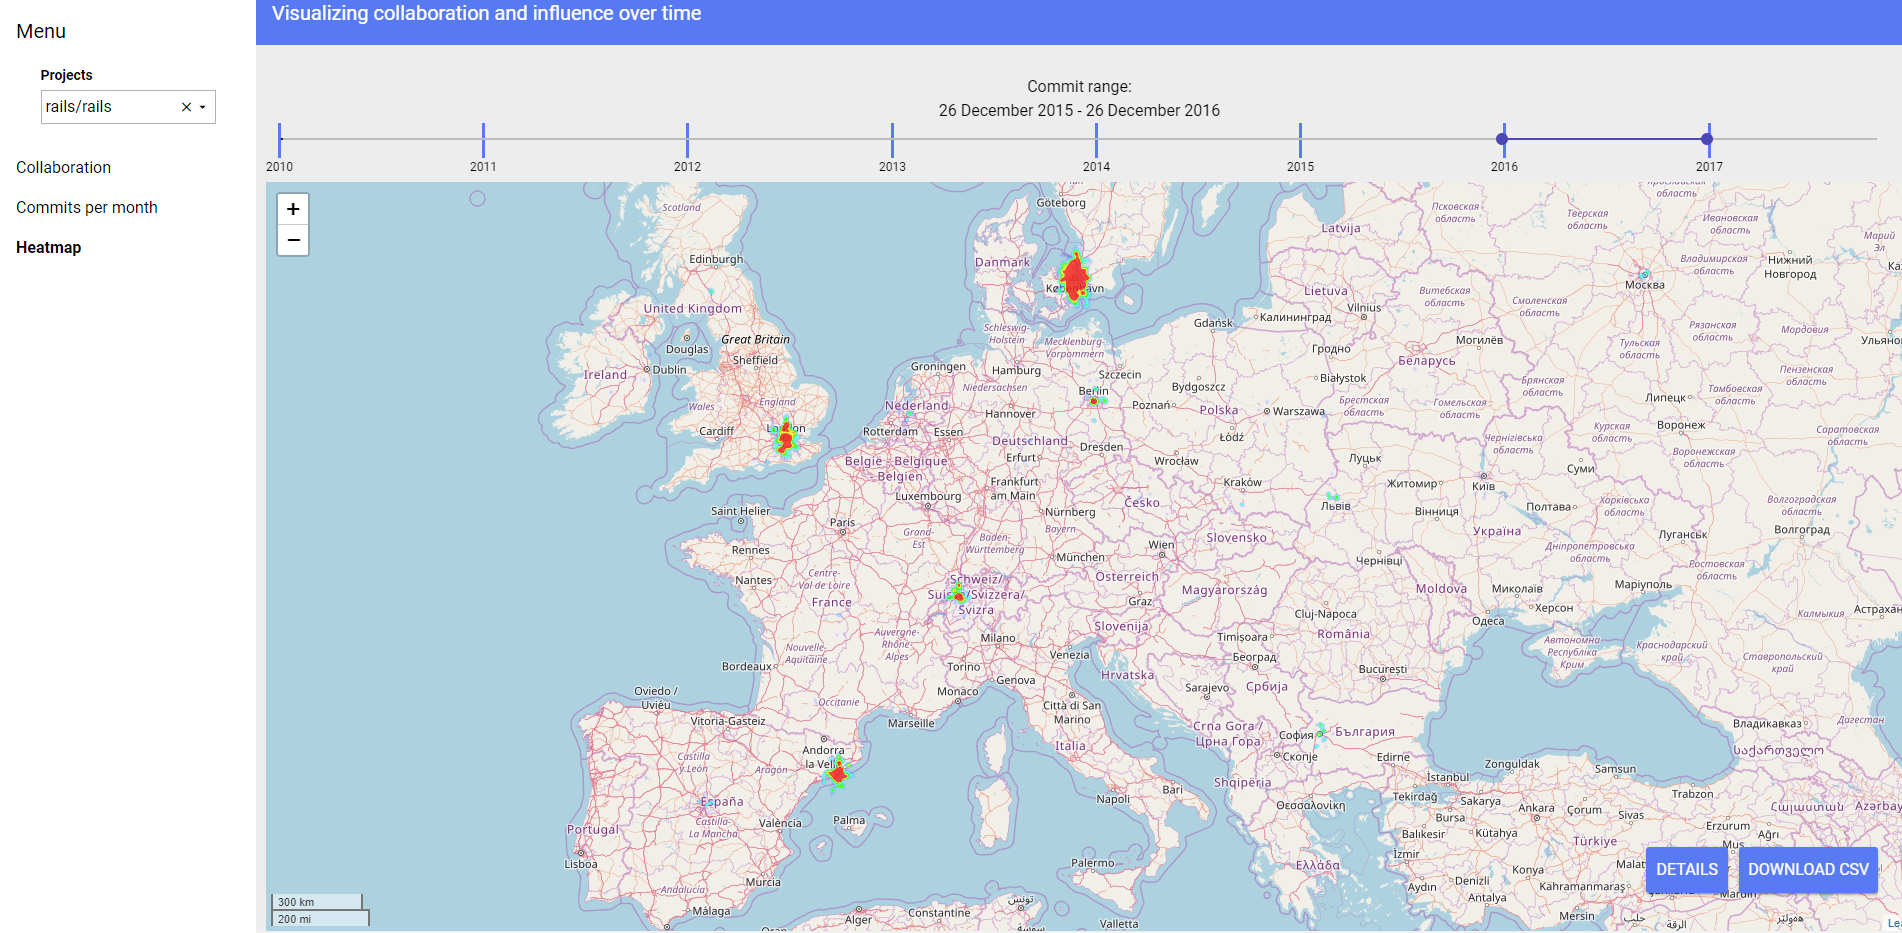
\includegraphics[scale=0.2]{images/rails-heatmap-2016-2017.PNG}
\caption{Example visualization of heatmap for rails from 2016 till 2017}
\label{fig:commits-heatmap}
\end{figure}

The third visualization in the application is a heatmap and is shown in figure ~\ref{fig:commits-heatmap}. 
As well as the visualization for commits per month, this visualization is created with the D3 library.
The heatmap visualization uses the same slider as the collaboration visualization.
The visualization creates a heatmap for the commits belonging to the selected timespan.
The heatmap visualizes commits by color ranging from green to red. 
Here red spots mean locations with a lot of commits, and green spots are locations with fewer commits.


Preliminary results contain 1000 repositories with over 5 million commits belonging to 160.000 users.
Not all of the user gave information on their whereabouts, but about 84.000 did.
This means that it was possible to retrieve locations for just over 50\% of the gathered users.

\section{Discussion}
Visualizing repository data is an interesting way of looking at the data from a different perspective. 
This leads to points of interest that otherwise wouldn't arise when looking at the raw data. 
By introducing location data to these visualizations one gets a good overview of  the geographic distribution of developers.

In the future, more types of visualizations can be added, as well as more interaction through the use of the D3 library.
In addition it would be of high value for stakeholders of a repository not listed in the used dataset to be able to import their repository in the web application itself, without having to resort to setup the project locally themselves.
\bibliographystyle{ACM-Reference-Format}
\bibliography{bibliography}

\end{document}


